\chapter{Learning Multi-Layer Dictionaries}
\section{Introduction}
A multi-layer dictionary model is composed of multiple dictionaries; the model treats the dictionary coefficients of a previous layer as the signal for the subsequent layer. This model dates back to Zeiler's Deconvolutional Neural Networks \cite{zeiler2010deconvolutional} and can be thought of as a deep autoencoder \cite[Chapter~14]{Goodfellow2016-DeepLearningBook}\cite{Rangamani2018DictLandAE}. Some researchers have interpreted convolutional neural networks as multi-layer dictionary models, the convolution and its corresponding rectified linear units serving as a crude pursuit algorithm \cite{papyan2017convolutional}. This chapter presents how to apply the novel dictionary learning algorithm from the prior chapter to the multi-layer dictionary learning problem.
\section{Literature Review}
In 2010, Zeiler et al. proposed a multi-layer dictionary model termed a deconvolutional network \cite{zeiler2010deconvolutional}. The learning process for dictionary filters is entirely unsupervised, and they learn their filters layer-by-layer. Their algorithm is greedy in the sense that there is no feedback from subsequent layers to influence the learning process on the previous layer. This approach was tested both on the task of removing added Gaussian noise to images, and also as a feature extraction method for object recognition on the Caltech-101 dataset \cite{fei2004-Caltech101}. While this research drew a lot of attention at the time, as the success of alternative models like convolutional neural networks grew \cite{krizhevsky2012imagenet}, the popularity of deconolutional networks decreased.

Multi-layer dictionaries also appear in Bayesian models, going by names such as hierarchical convolutional factor analysis \cite{chen2011hierarchical}\cite{chen2013deep} and deep deconvolutional learning \cite{pu2014generative}. These networks use probabilistic models to prune network architecture and provide interpretable dictionaries. Inference can be slow.

In more recent work, \cite{murdock2018deep} and \cite{chodosh2018deep} use ADMM for pursuit on a multi-layer dictionary model. Their pursuit algorithm attempts to solve the minimization problem:
\begin{equation}
\minimize_{\vx} = \sum_{\ell = 1}^{L} \frac{\mu_{\ell}}{2}\|\vx_{\ell - 1} -\mD_{\ell}\vx_{\ell}\|_2^2 + \lambda_{\ell}\|\vx_{\ell}\|_1
\end{equation}
where $\vx_0 = \vs$ is the signal. They convert this to a constrained optimization for the ADMM algorithm.
\begin{equation}
\begin{aligned}
\min_{\vx,\vz} & \sum_{\ell = 1}^{L} \frac{\mu_{\ell}}{2}\|\vz_{\ell - 1} -\mD_{\ell}\vx_{\ell}\|_2^2 + \lambda_{\ell}\|\vz_{\ell}\|_1 \\
\text{subject to } & \vz_{\ell} - \vx_{\ell} = 0
\end{aligned} \label{equation:ADMM Multi-Layer Pursuit Objective}
\end{equation}
where $\vz_0 = \vs$ is the signal. The $\vx$ updates involve solving an inverse problem. They use a tight-frame assumption to approximate the inverse.

Finally, in \cite{chodosh2020use}, Chodosh and Lucey use a similar model to \cite{murdock2018deep} and \cite{chodosh2018deep}, but replace the ADMM approach with FISTA-like linear-proximal iterative steps.

\section{Multi-Layer ADMM with Low-Rank Updates}
This chapter demostrates how to apply the novel sparse coding method for multi-channel signals to a multi-layer dictionary pursuit problem.

To start off, it is helpful to write a multi-layer dictionary optimization problem. To keep things compact, let $\vx_0 = \vs$. I use a similar multi-layer dictionary model to the one used in \cite{murdock2018deep} and \cite{chodosh2018deep}:
%
\begin{equation}
\minimize_{\vx} \sum_{\ell = 1}^{L} \frac{\mu_{\ell}}{2}\|\vx_{\ell - 1} -\mD_{\ell}\vx_{\ell}\|_2^2 + \lambda_{\ell}\|\vx_{\ell}\|_1
\end{equation}
%
Applying the ADMM algorithm, I add a secondary primal variable $\vz_{\ell}$ for each layer $\ell$ and constrain it to be equal to $\vx_{\ell}$. As in the previous chapter, I scale this constraint so that the inverse representation can be updated efficiently without losing the normalized quality of the dictionary. This replaces the tight-frame assumption used in \cite{murdock2018deep} and \cite{chodosh2018deep}. Again, keeping things compact, let $\vz_0 = \vs$.
%
\begin{equation}
\begin{aligned}
\min_{\vx,\vz} & \sum_{\ell = 1}^{L} \frac{\mu_{\ell}}{2}\|\vz_{\ell - 1} -\mD_{\ell}\vx_{\ell}\|_2^2 + \lambda_{\ell}\|\vz_{\ell}\|_1 \\
\text{subject to } & \sqrt{\mu_{\ell}}\mR_{\ell}^{-1}\vz_{\ell} - \sqrt{\mu_{\ell}}\mR_{\ell}^{-1}\vx_{\ell} = 0
\end{aligned}
\end{equation}
%
where $\vz_0 = \vs$ is not a primal variable, but instead the signal itself.

This optimization problem has the augmented Lagrangian function:
%
\begin{equation}
\L_{\rho}(\vx,\vz,\vgamma) = f(\vx,\vz)  +  \sum_{\ell = 1}^L \frac{\rho}{2}\|\sqrt{\mu_{\ell}}\mR_{\ell}^{-1}(\vz_{\ell} - \vx_{\ell}) + \frac{\vgamma_{\ell}}{\rho}\|_2^2  - \frac{\rho}{2}\|\frac{\vgamma_{\ell}}{\rho}\|_2^2
\end{equation}
%
where 
\begin{equation}
f(\vx,\vz) = \sum_{\ell = 1}^{L} \frac{\mu_{\ell}}{2}\|\vz_{\ell - 1} -\mD_{\ell}\vx_{\ell}\|_2^2 + \lambda_{\ell}\|\vz_{\ell}\|_1
\end{equation}

Recall that the ADMM algorithm (with relaxation) iteratively alternates between primal and dual updates, using four update equations:
\begin{equation} \label{equation:general x-update ADMM}
\vx^{(t + 1)} = \arg\min_{\vx} \L(\vx,\vz^{(t)},\vgamma^{(t)})
\end{equation}
%
\begin{equation}
\frac{\vgamma^{\left(t + \frac{1}{2}\right)}}{\rho} = \frac{\vgamma^{(t)}}{\rho} + (\alpha - 1)(\mA\vx^{(t + 1)} + \mB\vz^{(t)} + \vc)
\end{equation}
%
\begin{equation} \label{equation:general y-update ADMM}
\vz^{(t + 1)} = \arg\min_{\vz} \L\left(\vx^{(t + 1)},\vz,\vgamma^{\left(t + \frac{1}{2}\right)}\right)
\end{equation}
%
\begin{equation}
\frac{\vgamma^{(t + 1)}}{\rho} = \frac{\vgamma^{\left(t + \frac{1}{2}\right)}}{\rho} + \mA\vx^{(t + 1)} + \mB\vz^{(t + 1)} + \vc
\end{equation}
%
where $\mA\vx + \mB\vz + \vc = \vzero$ are the affine constraints.

The first of these updates is the $\vx$ update, which updates the coefficients.


\subsection{Coefficients Update Equation}
The coefficients update comes from equation \ref{equation:general x-update ADMM}, which can be derived through setting the gradient of the Lagrangian equal to zero and solving for $\vx$.
%
\begin{equation}
\nabla_{\vx_{\ell}} f(\vx,\vz) = \mu_{\ell}\mD_{\ell}^T\mD_{\ell}\vx_{\ell} - \mu_{\ell}\mD_{\ell}^T\vz_{\ell - 1}
\end{equation}
%
\begin{equation}
\nabla_{\vx_{\ell}} \frac{1}{2}\|\sqrt{\mu_{\ell}}\mR_{\ell}^{-1}(\vz_{\ell} - \vx_{\ell}) + \frac{\vgamma_{\ell}}{\rho}\|_2^2 = \mu_{\ell}\mR_{\ell}^{-2}\vx - \mu_{\ell}\mR_{\ell}^{-2}\vz_{\ell} - \frac{\sqrt{\mu_{\ell}}\mR_{\ell}^{-1}\vgamma_{\ell}}{\rho}
\end{equation}
%
Therefore,
%
\begin{equation}
\nabla_{\vx_{\ell}} \L_{\rho}(\vx,\vz,\vgamma) = \mu_{\ell}\mD_{\ell}^T\mD_{\ell}\vx_{\ell} - \mu_{\ell}\mD_{\ell}^T\vz_{\ell - 1} + \rho\left(\mu_{\ell}\mR_{\ell}^{-2}\vx - \mu_{\ell}\mR_{\ell}^{-2}\vz_{\ell} - \frac{\sqrt{\mu_{\ell}}\mR_{\ell}^{-1}\vgamma_{\ell}}{\rho}\right)
\end{equation}

For $\vx$, $\vz$, $\vgamma$, such that $\nabla_{\vx_{\ell}} \L_{\rho}(\vx_1,\hdots,\vx_L,\vz_1,\hdots,\vz_L,\vgamma_1,\hdots,\vgamma_L) = 0$:
%
\begin{equation}
\mu_{\ell}(\rho \mR_{\ell}^{-2} + \mD_{\ell}^T\mD_{\ell})\vx_{\ell} = \mu_{\ell}\mD_{\ell}^T\vz_{\ell - 1} + \rho \mu_{\ell}\mR_{\ell}^{-2}\vz_{\ell} + \sqrt{\mu_{\ell}}\mR_{\ell}^{-1}\vgamma_{\ell}
\end{equation}
%
\begin{equation}
(\rho \mR_{\ell}^{-2} + \mD_{\ell}^T\mD_{\ell})\vx_{\ell} = \mD_{\ell}^T\vz_{\ell - 1} + \rho \mR_{\ell}^{-2}\vz_{\ell} + \frac{\mR_{\ell}^{-1}\vgamma_{\ell}}{\sqrt{\mu_{\ell}}}
\end{equation}
%
\begin{equation}
\vx_{\ell} = (\rho \mR_{\ell}^{-2} + \mD_{\ell}^T\mD_{\ell})^{-1}\left(\mD_{\ell}^T\vz_{\ell - 1} + \rho \mR_{\ell}^{-2}\vz_{\ell} + \frac{\mR_{\ell}^{-1}\vgamma_{\ell}}{\sqrt{\mu_{\ell}}}\right)
\end{equation}
%
This solution is the $\vx$ update for the ADMM algorithm, but a couple extra steps can put it into a form that is easier to use.
%
\begin{equation}
\vx_{\ell} = \mR_{\ell}\left(\rho \mId + (\mD_{\ell}\mR_{\ell})^T\mD_{\ell}\mR_{\ell}\right)^{-1}\mR_{\ell}\left(\mD_{\ell}^T\vz_{\ell - 1} + \rho \mR_{\ell}^{-2}\vz_{\ell} + \frac{\mR_{\ell}^{-1}\vgamma_{\ell}}{\sqrt{\mu_{\ell}}}\right)
\end{equation}
%
\begin{equation}
\mR_{\ell}^{-1}\vx_{\ell} = \left(\rho \mId + (\mD_{\ell}\mR_{\ell})^T\mD_{\ell}\mR_{\ell}\right)^{-1}\left((\mD_{\ell}\mR_{\ell})^T\vz_{\ell - 1} + \rho \mR_{\ell}^{-1}\vz_{\ell} + \frac{\vgamma_{\ell}}{\sqrt{\mu_{\ell}}}\right)
\end{equation}
%
So, therefore the update equation for $\mR_{\ell}^{-1}\vx_{\ell}$ is the following:
%
\begin{equation} \label{equation:Multi-Layer x-Update Equation}
\mR_{\ell}^{-1}\vx_{\ell}^{(t + 1)} = \left(\rho \mId + (\mD_{\ell}\mR_{\ell})^T\mD_{\ell}\mR_{\ell}\right)^{-1}\left((\mD_{\ell}\mR_{\ell})^T\vz_{\ell - 1}^{(t)} + \rho \left(\mR_{\ell}^{-1}\vz_{\ell}^{(t)} + \frac{\vgamma_{\ell}^{(t)}}{\rho\sqrt{\mu_{\ell}}}\right)\right)
\end{equation}
%
Before moving onto another update equation, there are a few useful things to note here. The form of the inverse matrix identically matches the form from the last chapter, so the inverse representation can be updated efficiently if the updates have a low-rank structure. Furthermore, $\mD_{\ell}\mR_{\ell}$ is the unnormalized dictionary that is updated through low-rank updates. The normalized dictionary does not need to be explicitly calculated at all. It would be easy to isolate $\vx_{\ell}$, but it will be simpler to keep track of $\mR_{\ell}^{-1}\vx_{\ell}$ instead, similar to how $\frac{\vu}{\rho}$ is tracked instead of $\vu$ in the scaled ADMM algorithm.

\subsection{Proximal Updates}
The second set of primal updates comes from equation \ref{equation:general y-update ADMM}, repeated here for convenience:
\begin{equation}
\vz^{(t + 1)} = \arg\min_{\vz} \L\left(\vx^{(t + 1)},\vz,\vgamma^{\left(t + \frac{1}{2}\right)}\right)
\end{equation}
where, as before,
\begin{equation}
\L_{\rho}(\vx,\vz,\vgamma) = f(\vx,\vz)  +  \sum_{\ell = 1}^L \frac{\rho}{2}\|\sqrt{\mu_{\ell}}\mR_{\ell}^{-1}(\vz_{\ell} - \vx_{\ell}) + \frac{\vgamma_{\ell}}{\rho}\|_2^2  - \frac{1}{2\rho}\|\vgamma_{\ell}\|_2^2
\end{equation}
%
and
\begin{equation}
f(\vx,\vz) = \sum_{\ell = 1}^{L} \frac{\mu_{\ell}}{2}\|\vz_{\ell - 1} -\mD_{\ell}\vx_{\ell}\|_2^2 + \lambda_{\ell}\|\vz_{\ell}\|_1
\end{equation}

For $\vx$, $\vz$, $\vgamma$, such that $\nabla_{\vz_{\ell}} \L_{\rho}(\vx_1,\hdots,\vx_L,\vz_0,\hdots,\vz_L,\vgamma_0,\hdots,\vgamma_L) = 0$:
%
\begin{equation}
\nabla_{\vz} \frac{\mu_{\ell + 1}}{2}\|\vz_{\ell} - \mD_{\ell + 1}\vx_{\ell + 1}\|_2^2 + \lambda_{\ell}\|\vz_{\ell}\|_1 + \frac{\rho}{2} \|\sqrt{\mu_{\ell}}\mR_{\ell}^{-1}(\vz_{\ell} - \vx_{\ell}) + \frac{\vgamma_{\ell}}{\rho}\|_2^2 = 0
\end{equation}
%
Something important to note here is that each element of $\vz_{\ell}$ can be treated independently, that is:
%
\begin{equation}
\nabla_{\vz_{\ell}[i]} \frac{\mu_{\ell + 1}}{2}(\vz_{\ell}[i] - (\mD_{\ell + 1}\vx_{\ell + 1})[i])^2 + \lambda_{\ell}|\vz_{\ell}[i]| + \frac{\rho}{2} (\frac{\sqrt{\mu_{\ell}}}{\mR_{\ell}[i]}(\vz_{\ell}[i] - \vx_{\ell}[i]) + \frac{\vgamma_{\ell}[i]}{\rho})^2 = 0
\end{equation}
%
where $\mR{\ell}[i]$ is the scalar $i^{\text{th}}$ diagonal entry of diagonal matrix $\mR_{\ell}$.
%
\begin{equation}
\nabla_{\vz_{\ell}[i]} \frac{\mu_{\ell + 1}}{2}(\vz_{\ell}[i] - (\mD_{\ell + 1}\vx_{\ell + 1})[i])^2 + \lambda_{\ell}|\vz_{\ell}[i]| + \frac{\rho\mu_{\ell}}{2\mR_{\ell}^2[i]} (\vz_{\ell}[i] - \vx_{\ell}[i] + \frac{\mR_{\ell}[i]\vgamma_{\ell}[i]}{\rho\sqrt{\mu_{\ell}}})^2 = 0
\end{equation}
%
For the sake of brevity, I will now drop the indexing:
%
\begin{equation}
\nabla_{\vz_{\ell}} \frac{\mu_{\ell + 1}}{2}(\vz_{\ell}^2 - 2(\mD_{\ell + 1}\vx_{\ell + 1})z_{\ell}) + \lambda_{\ell}|\vz_{\ell}| + \frac{\rho\mu_{\ell}}{2\mR_{\ell}^2} (\vz_{\ell}^2 - 2\vx_{\ell}\vz_{\ell} + \frac{2\mR_{\ell}\vgamma_{\ell}\vz_{\ell}}{\rho\sqrt{\mu_{\ell}}}) = 0
\end{equation}
%
\begin{equation}
\nabla_{\vz_{\ell}} \frac{1}{2}(\mu_{\ell + 1} + \rho\mu_{\ell}\mR_{\ell}^{-2})\vz_{\ell}^2 - \mu_{\ell + 1}\mD_{\ell + 1}\vx_{\ell + 1}\vz_{\ell} - \rho\mu_{\ell}\mR_{\ell}^{-2}\vx_{\ell}\vz_{\ell} + \sqrt{\mu_{\ell}}\mR_{\ell}^{-1}\vgamma_{\ell}\vz_{\ell} + \lambda_{\ell}|\vz_{\ell}| = 0
\end{equation}
%
\begin{equation}
\nabla_{\vz_{\ell}} \frac{1}{2}\vz_{\ell}^2 - \frac{\mu_{\ell + 1}\mD_{\ell + 1}\vx_{\ell + 1} + \rho\mu_{\ell}\mR_{\ell}^{-2}\vx_{\ell} - \sqrt{\mu_{\ell}}\mR_{\ell}^{-1}\vgamma_{\ell}}{\mu_{\ell + 1} + \rho\mu_{\ell}\mR_{\ell}^{-2}}\vz_{\ell} + \frac{\lambda_{\ell}}{\mu_{\ell + 1} + \rho\mu_{\ell}\mR_{\ell}^{-2}}|\vz_{\ell}| = 0
\end{equation}
%
\begin{equation}
\vz_{\ell} = \operatorname{S}_{\frac{\lambda_{\ell}}{\mu_{\ell + 1} + \rho\mu_{\ell}\mR_{\ell}^{-2}}}\left(\frac{\mu_{\ell + 1}\mD_{\ell + 1}\vx_{\ell + 1} + \rho\mu_{\ell}\mR_{\ell}^{-2}(\vx_{\ell} - \frac{\mR_{\ell}\vgamma_{\ell}}{\rho\sqrt{\mu_{\ell}}})}{\mu_{\ell + 1} + \rho\mu_{\ell}\mR_{\ell}^{-2}}\right)
\end{equation}
%
\begin{equation}
\vz_{\ell} = \frac{1}{\mu_{\ell + 1} + \rho\mu_{\ell}\mR_{\ell}^{-2}}\operatorname{S}_{\lambda_{\ell}}\left(\mu_{\ell + 1}\mD_{\ell + 1}\vx_{\ell + 1} + \rho\mu_{\ell}\mR_{\ell}^{-1}\left(\mR_{\ell}^{-1}\vx_{\ell} - \frac{\vgamma_{\ell}}{\rho\sqrt{\mu_{\ell}}}\right)\right)
\end{equation}
%
\begin{equation}
\vz_{\ell}^{(t + 1)} = (\rho\mu_{\ell}\mId + \mu_{\ell + 1}\mR_{\ell}^2)^{-1}\mR_{\ell}^2\operatorname{S}_{\lambda_{\ell}}\left(\mu_{\ell + 1}\mD_{\ell + 1}\vx_{\ell + 1}^{(t + 1)} + \rho\mu_{\ell}\mR_{\ell}^{-1}\left(\mR_{\ell}^{-1}\vx_{\ell}^{(t + 1)} - \frac{\vgamma_{\ell}^{(t + \frac{1}{2})}}{\rho\sqrt{\mu_{\ell}}}\right)\right)
\end{equation}
%
Note there is a dependence on $\mR_{\ell + 1}^{-1}\vx_{\ell + 1}$. The last layer will have to be considered separately. Using the same procedure, the update for $\vz_L$ can be derived. Given how similar the derivations are to those used for the other $\vz$ layers, I will skip to the result.
%
%
\begin{equation}
\vz_L = \mR_{\ell}\operatorname{S}_{\frac{\lambda_L\mR_L}{\rho\mu_L}}\left(\mR_L^{-1}\vx_L - \frac{\vgamma_L}{\rho\sqrt{\mu_L}}\right)
\end{equation}
%
\begin{equation}
\vz_L^{(t + 1)} = \mR_{\ell}\operatorname{S}_{\frac{\lambda_L\mR_L}{\rho\mu_L}}\left(\mR_L^{-1}\vx_L^{(t + 1)} - \frac{\vgamma_L^{(t + \frac{1}{2})}}{\rho\sqrt{\mu_L}}\right)
\end{equation}

\subsection{Dual Updates}
Rather than tracking $\vgamma_{\ell}$ or $\frac{\vgamma_{\ell}}{\rho}$ explicitly, it will be easier to track $\frac{\vgamma_{\ell}}{\rho\sqrt{\mu_{\ell}}}$. The update equations are very straightforward.
%
\begin{equation}
\frac{\vgamma_{\ell}^{\left(t + \frac{1}{2}\right)}}{\rho\sqrt{\mu_{\ell}}} = \frac{\vgamma_{\ell}^{(t)}}{\rho\sqrt{\mu_{\ell}}} + (\alpha - 1)(\mR_{\ell}^{-1}\vz_{\ell}^{(t)} - \mR^{-1}\vx_{\ell}^{(t + 1)})
\end{equation}
%
\begin{equation}
\frac{\vgamma_{\ell}^{(t + 1)}}{\rho\sqrt{\mu_{\ell}}} = \frac{\vgamma_{\ell}^{\left(t + \frac{1}{2}\right)}}{\rho\sqrt{\mu_{\ell}}} + \mR_{\ell}^{-1}\vz_{\ell}^{(t + 1)} - \mR^{-1}\vx_{\ell}^{(t + 1)} 
\end{equation}

\section{Pursuit Algorithm Summary}
Together, the equations from the sections above produce a pursuit algorithm for a multi-layer dictionary model, as shown in algorithm \ref{algorithm:ADMM Multi-Layer Pursuit}. It is important to note that unlike in \cite{zeiler2010deconvolutional}, there is feedback between layers during pursuit.  Figure \ref{figure:ADMM Multi-Layer Pursuit Diagram} shows the interactions between layers across iterations. This allows for asymptotic convergence to an optimal solution of the objective in equation \ref{equation:ADMM Multi-Layer Pursuit Objective}.
\begin{figure}
	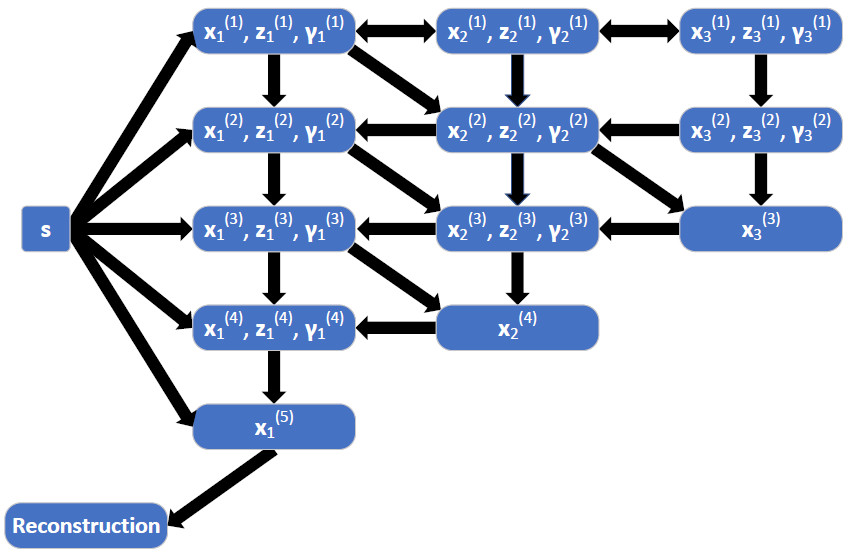
\includegraphics[width=\textwidth]{figures/multi-layer_ADMM-node-dependencies.PNG}
	\caption{This diagram shows interactions between layers across iterations. The double-sided arrows at the top of the diagram go both directions because $\vx_{\ell + 1}$ influences $\vz_{\ell}$ during initialization.}
	\label{figure:ADMM Multi-Layer Pursuit Diagram}
\end{figure}
\begin{algorithm}[h]
\SetAlgoLined 
\SetKwInOut{Input}{input}
\SetKwInOut{Output}{output}
\Input{Overrelaxation parameter: $\alpha \in (0,2]$, Number of layers: $L$, Number of filters: $M$, Signal size: $N$, Signal: $\vs$, Unnormalized dictionary for each layer: $\mD_{\ell}$, Objective function term coefficients: $\mu_{\ell}$ and $\lambda_{\ell}$, Efficient means to compute $(\rho\mId + \mD_{\ell}^T\mD_{\ell})^{-1}\vb$}
\Output{Sparse coding coefficients: either $\vx_{\ell}$ or $\vz_{\ell}$}
 %initialization:\\
   \For{$\ell \in \{1,\hdots, L\}$}
   {
      $\vgamma_{\ell} = \vzero$
      \For{$m \in \{1,\hdots, M\}$}
      {
         $r_{\ell}[m] = \|\mD_{\ell}[:,mN]\|_2$
      }
   }
   $\vx_1 = \mR_1^{-2} \mD_1^T$  \\
   \For{$\ell \in \{2,\hdots,L\}$}
   {
      $\vx_{\ell} = \mR_{\ell}^{-2}\mD_{\ell}^T\mR_{\ell - 1}\vx_{\ell - 1}$
   }
 \While{Not Converged}{
   \For{$\ell \in \{1,\hdots,L - 1\}$}
   {
      $\vz_{\ell} = (\rho\mu_{\ell}\mId + \mu_{\ell + 1}\mR_{\ell}^2)^{-1}\mR_{\ell}^2\operatorname{S}_{\lambda_{\ell}}\left(\mu_{\ell + 1}\mD_{\ell + 1}\vx_{\ell + 1} + \rho\mu_{\ell}\mR_{\ell}^{-1}(\vx_{\ell} - \vgamma_{\ell})\right)$
   }
   $\vz_L = \mR_L \operatorname{S}_{\frac{\lambda_L\mR_L}{\rho\mu_L}}(\vx_L - \vgamma_L)$ \\
   \For{$\ell \in \{1,\hdots,L\}$}
   {
      $\vgamma_{\ell} = \vgamma_{\ell} + \mR_{\ell}^{-1}\vz_{\ell} - \vx_{\ell}$
   }
   $\vx_1 = (\rho\mId + \mD_1^T\mD_1)^{-1}(\mD_1^T\vs + \rho(\mR_1^{-1}\vz_1 + \vgamma_1))$ \\
   \For{$\ell \in \{2,\hdots,L\}$}
   {
      $\vx_{\ell} = (\rho\mId + \mD_{\ell}^T\mD_{\ell})^{-1}(\mD_{\ell}^T\vz_{\ell - 1} + \rho(\mR_{\ell}^{-1}\vz_{\ell} + \vgamma_{\ell}))$
   }
   \For{$\ell \in \{1,\hdots,L\}$}
   {
      $\vgamma_{\ell} = \vgamma_{\ell} + (\alpha - 1)(\mR_{\ell}^{-1}\vz_{\ell} - \vx_{\ell})$
   }
 }
   \For{$\ell \in \{1,\hdots,L\}$}
   {
      $\vx_{\ell} = \mR_{\ell}\vx_{\ell}$
   }
 \caption{ADMM for Multi-Layer Pursuit with Unnormalized Dictionary}\label{algorithm:ADMM Multi-Layer Pursuit}
\end{algorithm}

\section{Dictionary Learning}
There are many possible approaches to compute dictionary updates, but the focus here will be on gradient descent. The pursuit algorithm generates several layers of coefficients from an input signal, and these coefficents can subsequently be used to generate some output, for classification, reconstruction, or some other task. With the appropriate choice of loss function $\loss$, backpropagation can be used to update the dictionaries. All of the computations in pursuit are almost\footnote{Like rectified linear activation functions, there is a discontinuity in the derivative for shrinkage operators. While such functions are technically not differentiable, this does not pose any issue for backpropagation. Operations that rely on a complex conjugate of a complex input also are not differentiable, but since the output is a scalar loss function, gradients can still be computed, which is sufficient for gradient descent. See Appendix C for details.} differentiable, so backpropagation is possible all the way back to the signal. Regardless of whether stochastic gradient descent or momentum methods such as Nesterov \cite{sutskever2013importance} or ADAM \cite{kingma2017adam} is used, the dictionary updates must be replaced with low-rank substitutes if the number of channels is large, so that the inverse decomposition can be updated efficiently. At least some of the gradients are computed in frequency domain. The convolutional filters are either spatially or temporally bound, and the frequency domain gradients will not respect that constraint, so they will need to be transformed and truncated.

Backpropagating gradients through most of the operations in the pursuit algorithm is very straightforward. Some platforms such as PyTorch \cite{paszke2017automatic} or TensorFlow \cite{tensorflow} will even do so automatically. However, the $\vx$-updates rely on a matrix decomposition to solve an inverse problem, and this prevents automatic differentiation in respect to the dictionaries. The equations necessary to compute gradients for the inverse problem in the $\vx$-update are derived in appendix C.
Let $\hat{\mD}_{\ell}$ be the frequency domain representation of the unnormalized dictionary corresponding to the $\ell$th layer, and let $\mQ_{\ell} = \rho\mId + \hat{\mD}_{\ell}^H\hat{\mD}_{\ell}$.
\begin{equation}
\nabla_{\hat{\mD}_{\ell}}^{(\vb \rightarrow \mQ_{\ell}^{-1}\vb)} \loss = -(\hat{\mD}_{\ell}\mQ_{\ell}^{-1}\vb)(\mQ_{\ell}^{-1}\nabla_{\mQ_{\ell}^{-1}\vb} \loss)^H - (\hat{\mD}_{\ell}\mQ_{\ell}^{-1}\nabla_{\mQ_{\ell}^{-1}\vb} \loss) (\mQ_{\ell}^{-1}\vb)^H
\end{equation}
where $\vb$ is the input vector to the computational step $\mQ_{\ell}^{-1}\vb$.\footnote{$\vb$ would take on a value like $\vb = \F\left((\mD_{\ell}\mR_{\ell})^T\vz_{\ell - 1}^{(t)} + \rho \left(\mR_{\ell}^{-1}\vz_{\ell}^{(t)} + \frac{\vgamma_{\ell}^{(t)}}{\rho\sqrt{\mu_{\ell}}}\right)\right) $, as seen in the $\vx$-update equation \ref{equation:Multi-Layer x-Update Equation}.} The superscript of the gradient specifies which gradient term is being computed. This is necessary because same dictionary gets reused across multiple computations, and so these gradient terms must be computed separately and then aggregated to get the actual gradient.

For the Woodbury form\footnote{Useful if the number of filters is larger than the number of channels}, the decomposition represents a different matrix for efficiently solving the inverse problem, and so the equation for the corresponding gradient term is different.
Let $\mXi_{\ell} = \rho\mId + \hat{\mD}_{\ell}\hat{\mD}_{\ell}^H$.
\begin{equation}
\nabla_{\hat{\mD}_{\ell}}^{(\vb \rightarrow \mXi_{\ell}^{-1}\vb)} \loss = -(\mXi_{\ell}^{-1}\nabla_{\mQ_{\ell}^{-1}\vb} \loss)(\hat{\mD}_{\ell}^H\mXi_{\ell}^{-1}\vb)^H -  (\mXi_{\ell}^{-1}\vb)(\hat{\mD}_{\ell}^H\mXi_{\ell}^{-1}\nabla_{\mQ_{\ell}^{-1}\vb} \loss)^H
\end{equation}
where $\vb$ is the input vector to the computational step $\mXi_{\ell}^{-1}\vb$.

With these equations it is possible to compute dictionary updates through backpropagation.  Putting it all together, a dictionary learning algorithm for multi-layer dictionary models is shown in algorithm \ref{algorithm:Multi-Layer Dictionary Learning}.

\begin{algorithm}[h]
\SetAlgoLined
   \SetKwInOut{Input}{input}
   \SetKwInOut{Output}{output}
   \Input{Overrelaxation Parameter: $\alpha \in (0,2]$, Signal: $\vs$, Unnormalized initial dictionary for each layer: $\mD_{\ell}$, Objective function term coefficients for each layer: $\mu_{\ell}$ and $\lambda_{\ell}$}
   \Output{Unnormalized dictionaries for each layer: $\mD_{\ell}$}
 %initialization:\\
   \For{$\ell \in \{1,\hdots,L\}$}
   {
      $\left(\rho\mId + \mD_{\ell}^T\mD_{\ell}\right) = \operatorname{ComputeDecomp}\left(\rho,\mD_{\ell} \right)$
   }
   $i = 0$ \\
   \While{Stopping Criteria Not Met}{
   $\vs = \operatorname{GetData}(i)$ \\
   $i = i + 1$ \\
   $\vx_1,\hdots,\vx_L = \operatorname{MultiLayerPursuit}(\vs,\alpha,\vmu,\vlambda,\mD,(\rho\mId + \mD_1^T\mD_1),\hdots,(\rho\mId + \mD_L^T\mD_L))$ \\
   $\loss = \operatorname{ComputeLoss}(\vx_1,\hdots,\vx_L)$ \\
   $\nabla_{\hat{\mD}_1} \loss,\hdots,\nabla_{\hat{\mD}_L} \loss = \operatorname{Backpropagation}(\loss,\mD_1,\hdots,\mD_L)$ \\
   $\mDelta \hat{\mD}_1,\hdots,\mDelta \hat{\mD}_L = \operatorname{CalculateGradientStep}(\nabla_{\hat{\mD}_1} \loss,\hdots,\nabla_{\hat{\mD}_L} \loss)$ \\
   \For{$\ell \in \{1,\hdots,L\}$}
   {
      $\tilde{\mD} = \operatorname{Normalize}(\hat{\mD}_{\ell} + \mDelta \hat{\mD}_{\ell})$ \\
      $\mDelta \mD_{\ell} = \operatorname{Truncate}(\F^{-1}\operatorname{RandomizedSVD}(\tilde{\mD} - \hat{\mD}_{\ell}))$ \\
      $\left(\rho\mId + \mD_{\ell}^T\mD_{\ell}\right) = \operatorname{UpdateDecomp}\left(\left(\rho\mId + \mD_{\ell}^T\mD_{\ell}\right),\rho,\mD_s,\mDelta\mD \right)$ \\
      $\mD_{\ell} = \mD + \mDelta\mD$ \\
      $\hat{\mD}_{\ell} = \F(\mD_{\ell})$
   }
   }
 \caption{Multi-Layer Dictionary Learning}\label{algorithm:Multi-Layer Dictionary Learning}
\end{algorithm}

\section{Summary}
In this chapter, I have applied the novel sparse coding algorithm from the previous chapter to a multi-layer dictionary model. If the dictionaries are updated with low-rank updates, the inverse representation necessary for the $\vx$ updates in the algorithm can be updated efficiently. This approach offers an alternative to direct proximal methods such as FISTA or mathematically suspect inverse approximations like the tight-frame assumption.
